\documentclass[11pt]{article}
\usepackage{tikz}
\usetikzlibrary{shapes, arrows}
\usepackage[hmargin=1in,vmargin=1in]{geometry}
\usepackage{xcolor}
\usepackage{enumitem} 
\usepackage{wrapfig}
\usepackage{amsmath,amssymb,amsfonts,url,sectsty,framed,tcolorbox,framed}
\newcommand{\pf}{{\bf Proof: }}
\newtheorem{theorem}{Theorem}
\newtheorem{lemma}{Lemma}
\newtheorem{proposition}{Proposition}
\newtheorem{definition}{Definition}  
\newtheorem{remark}{Remark}
\newcommand{\qed}{\hfill \rule{2mm}{2mm}}
\usepackage{fixltx2e}
\usepackage{graphicx}


\begin{document}
	%%%%%%%%%%%%%%%%%%%%%%%%%%%%%%%%%%%%%%%%%%%%%%%%%%%%%%%%%%%%%%%%%%%%%
	\noindent
	\rule{\textwidth}{1pt}
	\begin{center}
		{\bf [CS304] Introduction to Cryptography and Network Security}
	\end{center}
	Course Instructor: Dr. Dibyendu Roy \hfill Winter 2022-2023\\
	Scribed by: Pallikonda Sai Teja \hfill Lecture (Week 01)\\
	Student ID : 202011052
	\\
	\rule{\textwidth}{1pt}
	%%%%%%%%%%%%%%%%%%%%%%%%%%%%%%%%%%%%%%%%%%%%%%%%%%%%%%%%%%%
	%write here
	\section{Hill Cipher} 
	\\ 
	A = (a\textsubscript{ij})\textsubscript{nxn} \hspace{0.2cm} $\Rightarrow$ Invertable matrix \hspace{0.2cm} a\textsubscript{ij} \in Z\textsubscript{26}\\
	A $\Rightarrow$ Secret Key\\
	M = (m\textsubscript{1}m\textsubscript{2}....m\textsubscript{n})\\
	\subsection{Encryption}
	\begin{center}
		C = A.M = (c\textsubscript{1}c\textsubscript{2}....c\textsubscript{n})(mod26)
	\end{center}
	\subsection{Decryption}
	\begin{center}
		M = $A^{-1}$.C(mod26)
	\end{center}
	S = \{A,B,..,Z\} $\Rightarrow$ \{A,B,..,Z\}\\
	P $\Rightarrow$ C = S(P) \hspace{0.2cm} C $\Rightarrow$ Known, S $\Rightarrow$ Secret key\\
	S = $26^{26}$ nearly equal to $2^{122}$ \\
	\section{Kerchoff's Rule}
	Design has to be public\\
	\section{Shannon's notion of perfect secrecy}
	E $\Rightarrow$ Encryption Algorithm\hfill E(M) = C $\Rightarrow$ Going via public channel\\
	M $\Rightarrow$ Message\\
	C $\Rightarrow$ Ciphertext\\
	\vspace{0.1cm}
	E will be providing perfect secrecy iff the ciphertext does not reveal any information regarding the plain text/message.\vspace{0.1cm}\\
	Pr[M = m,C = c] = Pr[M = m]\\
	Pr[message with ciphertext] = Pr[meassage]\\
	OTP $\Rightarrow$ One Time Pad
	\section{Symmetric Key Cipher}
	\begin{enumerate}
		\item Block Cipher
		\item Stream Cipher
	\end{enumerate}
	\subsection{Block Cipher}
	M = m\textsubscript{0}\textit{$||$m\textsubscript{1}$||$...$||$m\textsubscript{l}}\\
	The plain text is divided into blocks and each block is encrypted and decrypted using the same key.
	\subsection{Stream Cipher}
	M = m\textsubscript{0}m\textsubscript{1}...m\textsubscript{l}\\
	In stream cipher bitwise encryption will be done.\\
	Stream cipher is used to encrypt the long messages.
	\section{Product cipher}
	
	
	\subsection{Substitution Permutation Network SPN}
	It is a product cipher based on Substitution box and Permutation box.\\ 
	In each round successively a substitution function and a permutation function on the lm bit input to that found are applied.
	
	Example  S : $\{0,1\}^n$ $\Rightarrow$ $\{0,1\}^m$, P : \{0,1,..,mr-1\} $\Rightarrow$ \{0,1,..,mr-1\}
	
	length(input) = n*r
	
	\subsection{Feistel Networrk}
	\begin{enumerate}
		\item In Feistel network, the plain text is of size 2n bits will be there.
		\item A Feistel network uses a round function, it will take two inputs – a data block and a subkey – and returns one output of the same size as the data block. 
		\item Round function(f) may not be invertible but still you can decrypt.
		\item The function associated to the feistel cipher in one round is invertible, no matter what is the property of one function 'f'.
	\end{enumerate}
	f : $\{0,1\}^n$ x $\{0,1\}^l$ $\rightarrow$ $\{0,1\}^n$\\
	2n $\rightarrow$ Length of plain text\\
	l $\rightarrow$ Bits in key\\
	\textbf{Encryption :}\vspace{0.1cm}\\
	\begin{center}
		\includegraphics[width=3cm]{encryption.jpg} \vspace{0.2cm}\\
	\end{center}
	L\textsubscript{1} = R\textsubscript{0}\\
	R\textsubscript{1} = L\textsubscript{0} $\oplus$ f(R\textsubscript{0},k)\\
	\textbf{Decryption :}\vspace{0.1cm}\\
	\begin{center}
		\includegraphics[width=3cm]{decryption.jpg} \vspace{0.2cm}\\
	\end{center}
	R\textsubscript{0} = L\textsubscript{1}\\
	L\textsubscript{0} = R\textsubscript{1} $\oplus$ f(L\textsubscript{1},k)\\
	\section{Iterated Block Cipher}
	
	\begin{enumerate}
		\item An iterated block cipher is block cipher involving the sequential repetition of an internal function(called as round function).
		\item The parameters include the number of rounds r, the block size n, and the round keys k\textsubscript{i} of length l generated from the original secret key k.
		\item Iterated Block Cipher, the number of keys used will be more and encryption will be done based on number of rounds. 
		\item In this key scheduling function will be there that will generate the round keys.
	\end{enumerate} 
	Example \\
	F $\Rightarrow$ Round Function\\
	P $\Rightarrow$ Plaintext block\\
	K  $\Rightarrow$ Secret Key\vspace{0.1cm}\\
	\begin{center}
		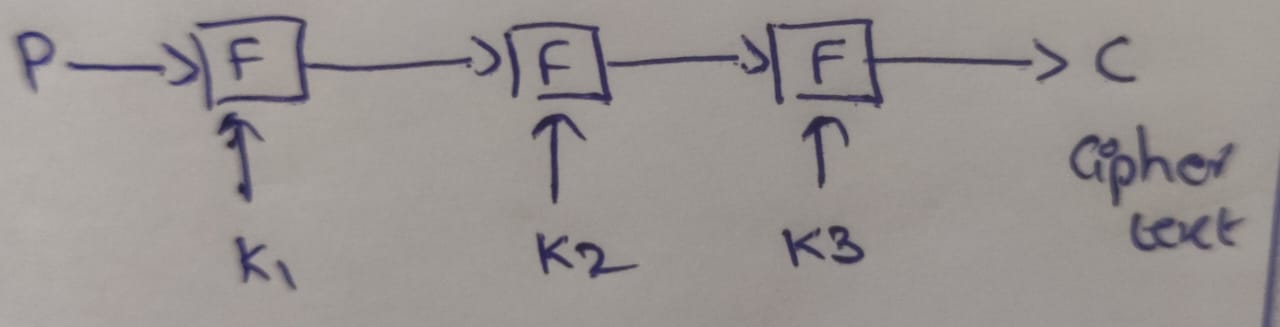
\includegraphics[width = 7cm]{IBC.jpg}\vspace{0.1cm}\\
	\end{center}
	G(k) $\Rightarrow$ k\textsubscript{1},k\textsubscript{2},k\textsubscript{3} $\Rightarrow$ Round Keys\\
	G(k) $\Rightarrow$ Key Scheduling function 
	\section{One Time Padding} 
	\begin{itemize} 
		\item One time padding provides the perfect secrecy under some conditions:
		\begin{enumerate}
			\item Condition-1: We cannot reuse the key to encrypt two messages.
			\item Condition-2: Length of key is greater than length of plain text.
			\item Condition-3: The key k is uniformly selected from the key space.
		\end{enumerate}
	\end{itemize}
	P $\Rightarrow$ Plain Text\\
	K $\Rightarrow$ Secret Key\vspace{0.2cm}\\
	Encryption(P,k) = P $\oplus$ k = C\\
	Decryption(C,k) = C $\oplus$ k = P
	
\end{document}
